\documentclass[11pt, a4paper]{article}
\usepackage{pdfpages}
\usepackage{parallel}
\usepackage[T2A]{fontenc}
%\usepackage{ucs}
\usepackage[utf8]{inputenc}
\usepackage[english,russian]{babel}
\usepackage{hyperref}
\usepackage{rotating}
\usepackage[inner=2cm,top=1.8cm,outer=2cm,bottom=2.3cm,nohead]{geometry}
%\usepackage{listings}
\usepackage{graphicx}
\usepackage{wrapfig}
\usepackage{longtable}
\usepackage{indentfirst}
\usepackage{array}
\usepackage{tikzsymbols}
\usepackage{soul}
\usepackage[ruled,vlined]{algorithm2e}
\usepackage{qrcode}
\counterwithout{figure}{section} 

\usepackage{url}
\makeatletter
\g@addto@macro{\UrlBreaks}{\UrlOrds}
\makeatother

\newcolumntype{P}[1]{>{\raggedright\arraybackslash}p{#1}}
\frenchspacing
%\usepackage{fixltx2e} %text sub- and superscripts
\usepackage{icomma} % коскі ў матэматычным рэжыме
%\PreloadUnicodePage{4}

\newcommand{\longpage}{\enlargethispage{\baselineskip}}
\newcommand{\shortpage}{\enlargethispage{-\baselineskip}}

\def\switchlang#1{\expandafter\csname switchlang#1\endcsname}
\def\switchlangbe{
\let\saverefname=\refname%
\def\refname{Літаратура}%
\def\figurename{Іл.}%
}
\def\switchlangru{
\let\saverefname=\refname%
\let\savefigurename=\figurename%
\def\refname{Литература}%
\def\figurename{Рис.}%
}
\def\switchlangen{
\let\saverefname=\refname%
\def\refname{References}%
\def\figurename{Fig.}%
}

\hyphenation{admi-ni-stra-tive}
\hyphenation{ex-pe-ri-ence}
\hyphenation{fle-xi-bi-li-ty}
\hyphenation{Py-thon}
\hyphenation{ma-the-ma-ti-cal}
\hyphenation{re-ported}
\hyphenation{imp-le-menta-tions}
\hyphenation{pro-vides}
\hyphenation{en-gi-neering}
\hyphenation{com-pa-ti-bi-li-ty}
\hyphenation{im-pos-sible}
\hyphenation{desk-top}
\hyphenation{elec-tro-nic}
\hyphenation{com-pa-ny}
\hyphenation{de-ve-lop-ment}
\hyphenation{de-ve-loping}
\hyphenation{de-ve-lop}
\hyphenation{da-ta-ba-se}
\hyphenation{plat-forms}
\hyphenation{or-ga-ni-za-tion}
\hyphenation{pro-gramming}
\hyphenation{in-stru-ments}
\hyphenation{Li-nux}
\hyphenation{sour-ce}
\hyphenation{en-vi-ron-ment}
\hyphenation{Te-le-pathy}
\hyphenation{Li-nux-ov-ka}
\hyphenation{Open-BSD}
\hyphenation{Free-BSD}
\hyphenation{men-ti-on-ed}
\hyphenation{app-li-ca-tion}

\def\progref!#1!{\texttt{#1}}
\renewcommand{\arraystretch}{2} %Іначай формулы ў матрыцы зліпаюцца з лініямі
\usepackage{array}

\def\interview #1 (#2), #3, #4, #5\par{

\section[#1, #3, #4]{#1 -- #3, #4}
\def\qname{LVEE}
\def\aname{#1}
\def\q ##1\par{{\noindent \bf \qname: ##1 }\par}
\def\a{{\noindent \bf \aname: } \def\qname{L}\def\aname{#2}}
}

\def\interview* #1 (#2), #3, #4, #5\par{

\section*{#1\\{\small\rm #3, #4. #5}}
\ifx\ParallelWhichBox\undefined%
    \addcontentsline{toc}{section}{#1, #3, #4}%
\else%
\ifnum\ParallelWhichBox=0%
    \addcontentsline{toc}{section}{#1, #3, #4}%
\fi\fi%

\def\qname{LVEE}
\def\aname{#1}
\def\q ##1\par{{\noindent \bf \qname: ##1 }\par}
\def\a{{\noindent \bf \aname: } \def\qname{L}\def\aname{#2}}
}

\newcommand{\interviewfooter}[1]{
\vskip 1em
\noindent \textit{#1}
}

\AtEndDocument{\vfill\centering \qrcode{https://github.com/fiowro/mouses/blob/main/\jobname.pdf}}

\switchlang{en}
\begin{document}

\title{1988 -- Asher Turbo trackball}
\date{}
\maketitle
\selectlanguage{english}
The Asher Turbo trackball shown in fig. \ref{fig:AsherPic} is a device for Apple Macintosh computers with the ADB bus. It is developed based on the quadLYNX trackball -- a member of the LX200 trackballs family. LX200 trackballs, better known by their microLYNX and comLYNX variants, were released in California by Honeywell, a subsidiary of Disc Instruments; they proved to be a long-lived family of products, with many subsequent reissues under different brands, differentiating by connection interfaces and electronics \cite{lx200}. Judging by the advertising materials, the quadLYNX model under the Honeywell brand appeared in 1986 \cite{honeywell}. Following that, in 1988 two new trackballs had appeared under the Asher Engineering Corporation brand: the quadLYNX ``LX200-192-D1'' (mentioning Honeywell as the original developer of the device) \cite{asher}, and Turbo Trackball ``LX200-192-S3A'' in a differently shaped case, but with a strong similarity in some internal design solutions \cite{turbo}.

\begin{figure}[h]
    \centering
    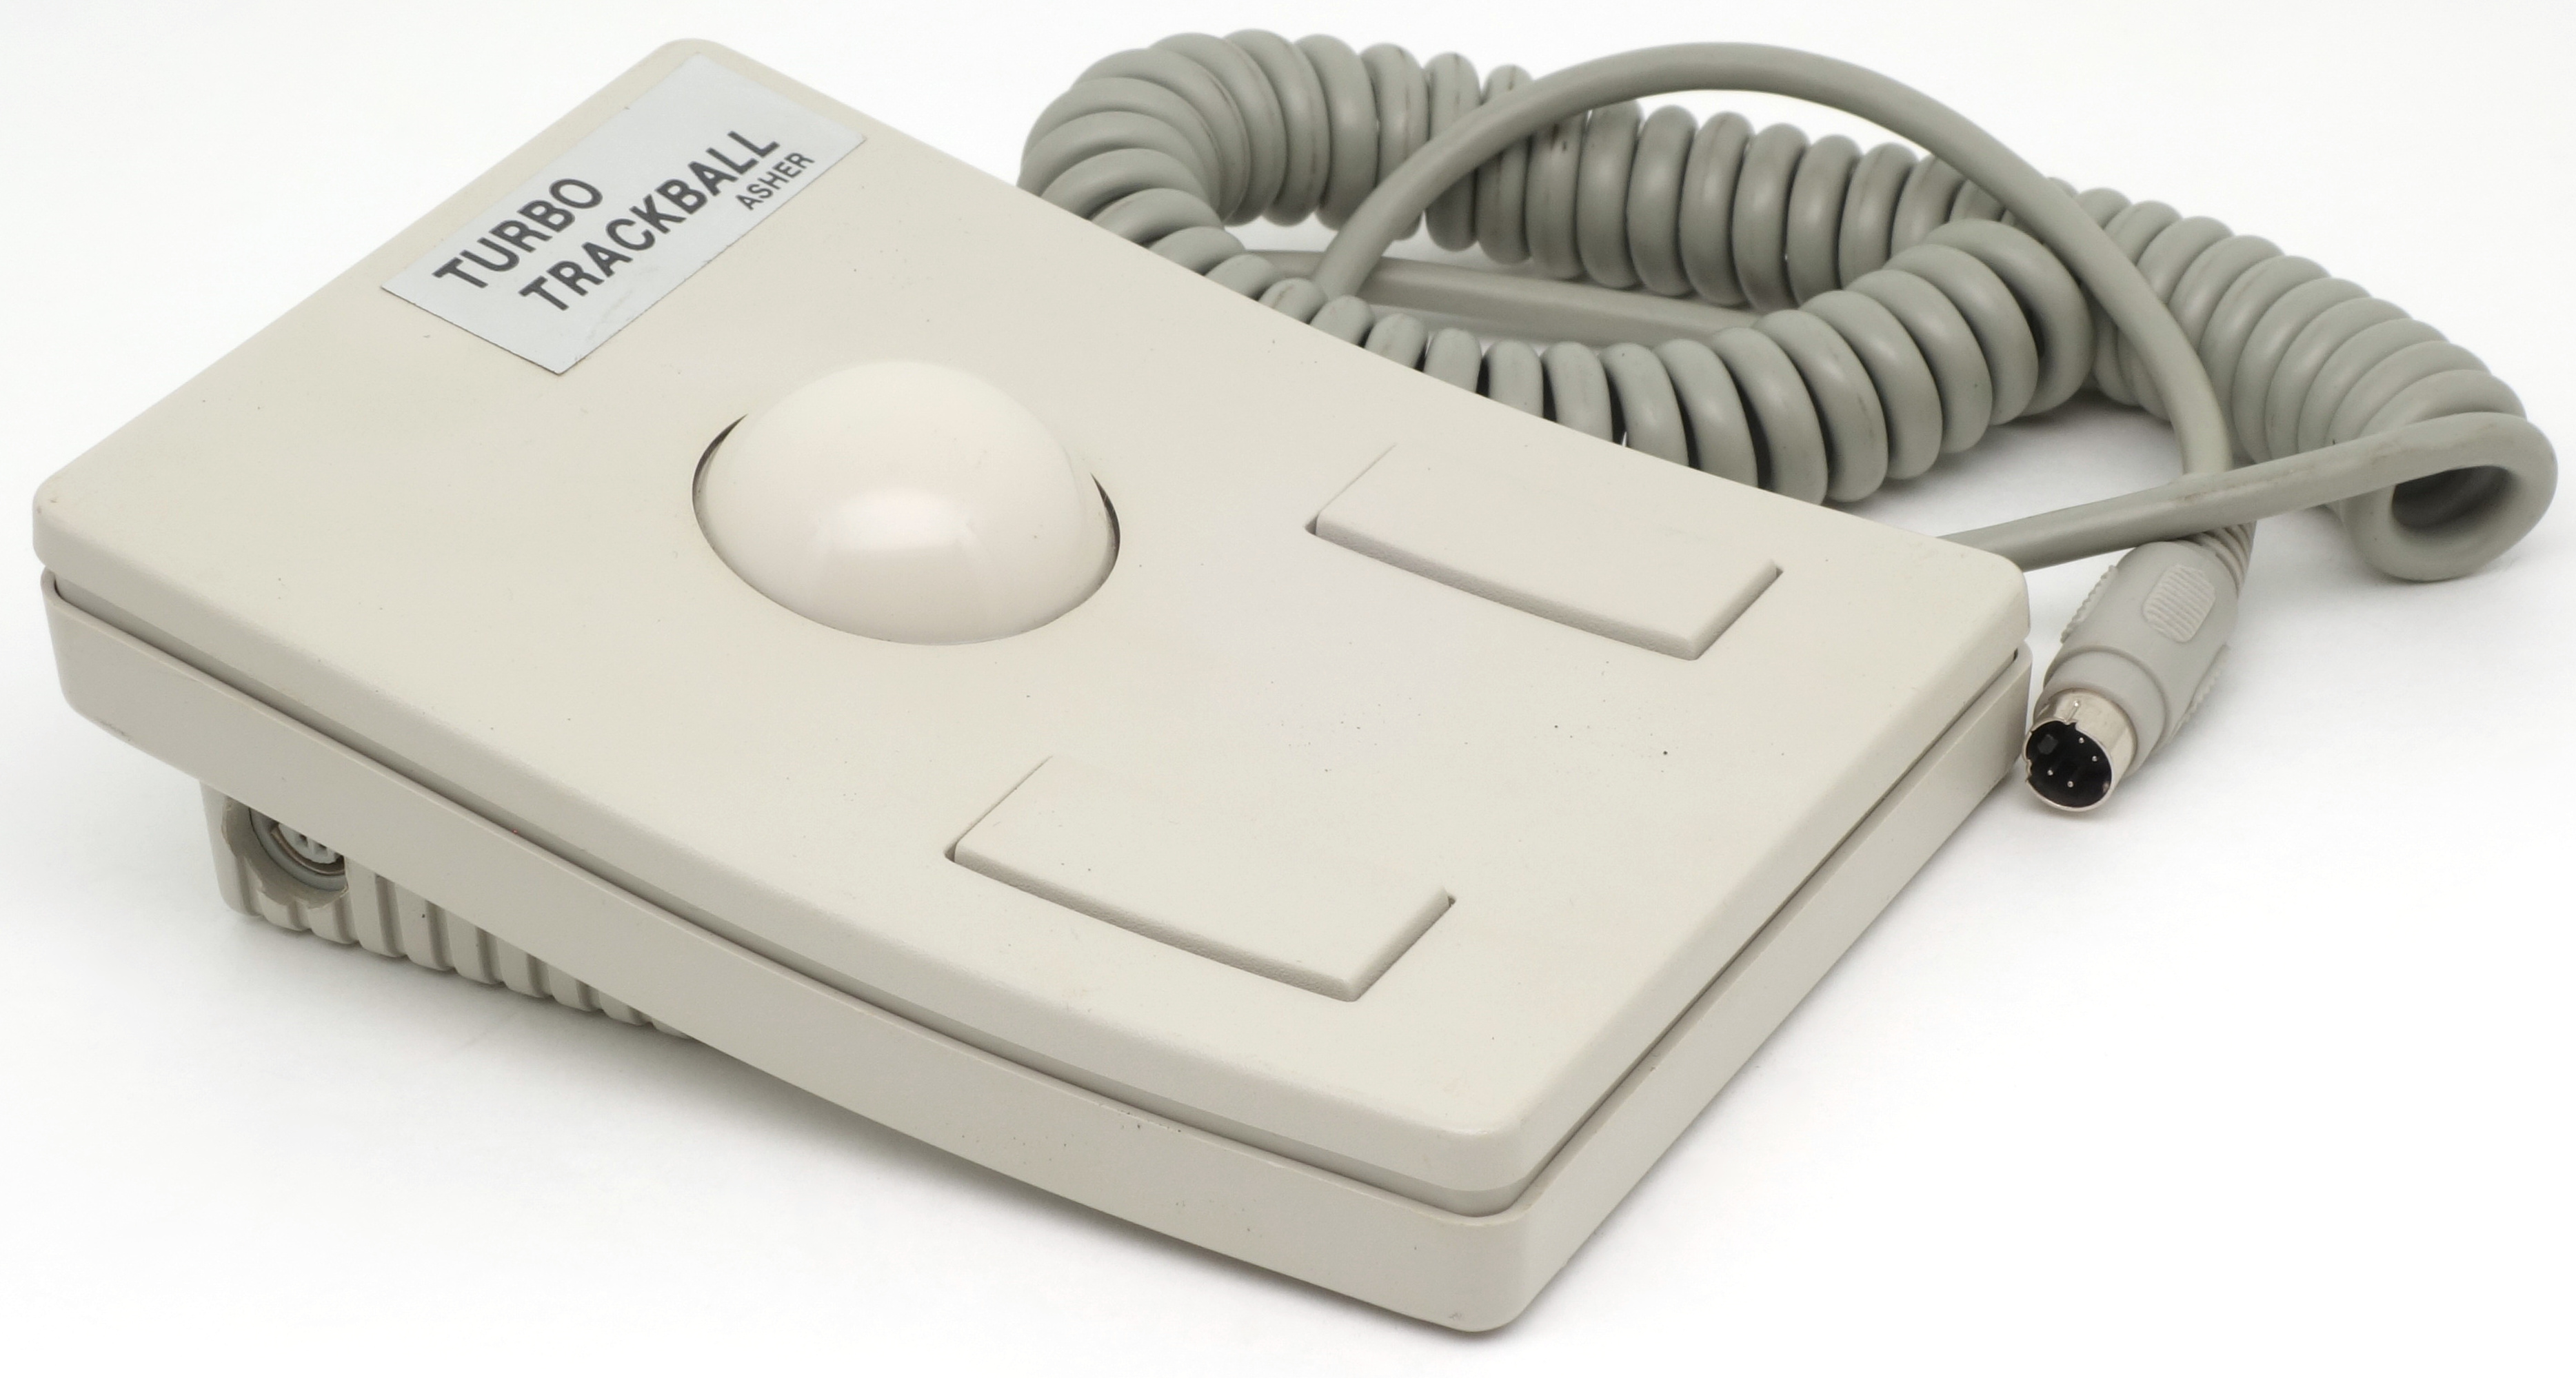
\includegraphics[width=\textwidth]{1988_asher_turbo_trackball/pic_60.jpg}
    \caption{Asher Turbo trackball}
    \label{fig:AsherPic}
\end{figure}

Unlike the typical design of the LX200 models, the Asher Turbo is made in a case, the upper side of which is inclined towards the user and slightly concave, repeating the profile of computer keyboards of that time (fig. \ref{fig:AsherTopBottom}). Two rectangular buttons, located in front of the ball on the side closest to the user, are flat, slightly protruding from the case, and their large area is beneficial for the ergonomics of the device. The left button functions as the main mouse button (or rather, the only one, given the specifics of the Apple ecosystem), and the right one functions as a drag ``latch''. Pressing the latch button virtually fixes the main trackball button in the pressed position, and pressing either button again turns off this mode.

The manufacturer positioned this trackball as a ``versatile, reliable, easy to use and very accurate device for sophisticated desktop publishing, graphics, CADCAM and many other applications''. In particular, it was emphasized that all advertising for this trackball, including illustrations, was desktop-published using the Asher Turbo trackball \cite{turbo}.

\begin{figure}[h]
    \centering
    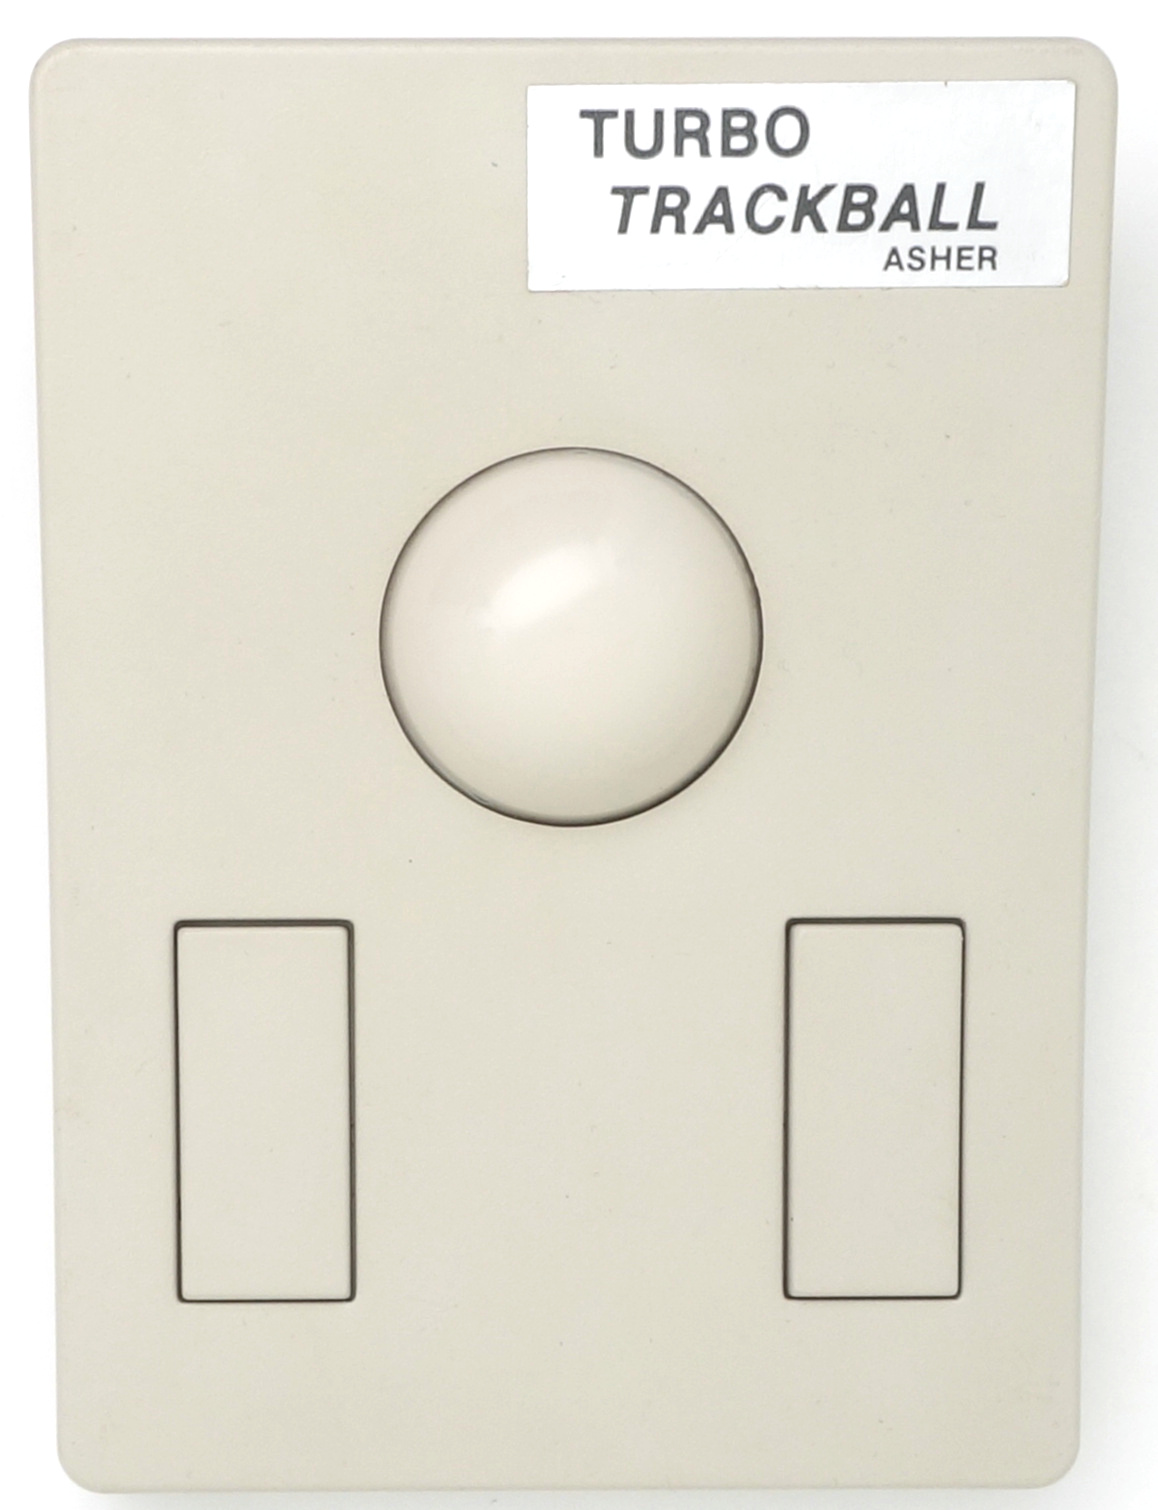
\includegraphics[scale=0.65]{1988_asher_turbo_trackball/top_15.jpg}
    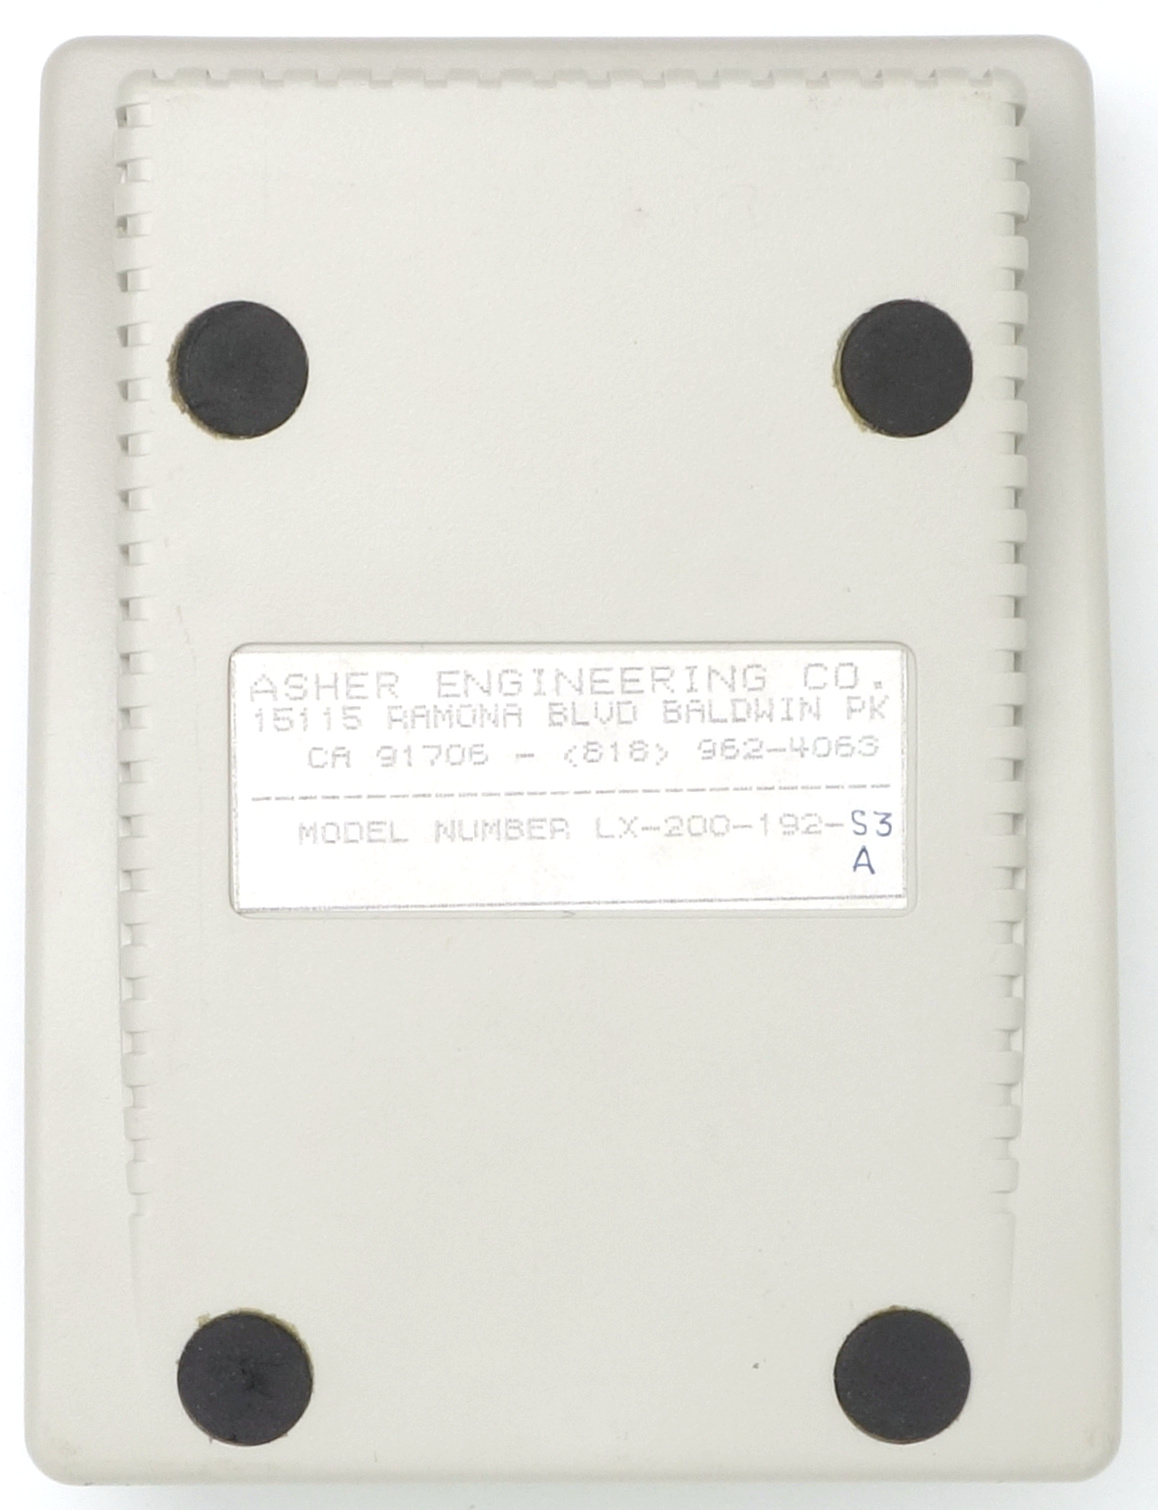
\includegraphics[scale=0.65]{1988_asher_turbo_trackball/bottom_15.jpg}
    \caption{Asher Turbo trackball, top and bottom views}
    \label{fig:AsherTopBottom}
\end{figure}

The trackball dimensions are smaller than traditional LX200 models, as they are dictated by the dimensions of the computer keyboard, for which the trackball should be a functional extension, located to the side of it. In general, this position should create fairly comfortable working conditions (fig. \ref{fig:AsherSize}).

The ads highlighted the Asher trackball's advantages over two models of relatively the same form-factor, the Abaton ProPoint and the Kensington Turbo Mouse, noticing it's higher resolution (250 CPI vs. 200 CPI) for more precise cursor control, and a compact, low profile, ergonomic package. Unlike the optomechanical design used in the Abaton and Kensington trackballs, Asher touted its unique ``patented high-tech encoder used in sophisticated aerospace instrumentation; like aircraft, missiles, torpedos, gyros, and space shuttles'' \cite{turbo}.

\begin{figure}[h]
    \centering
    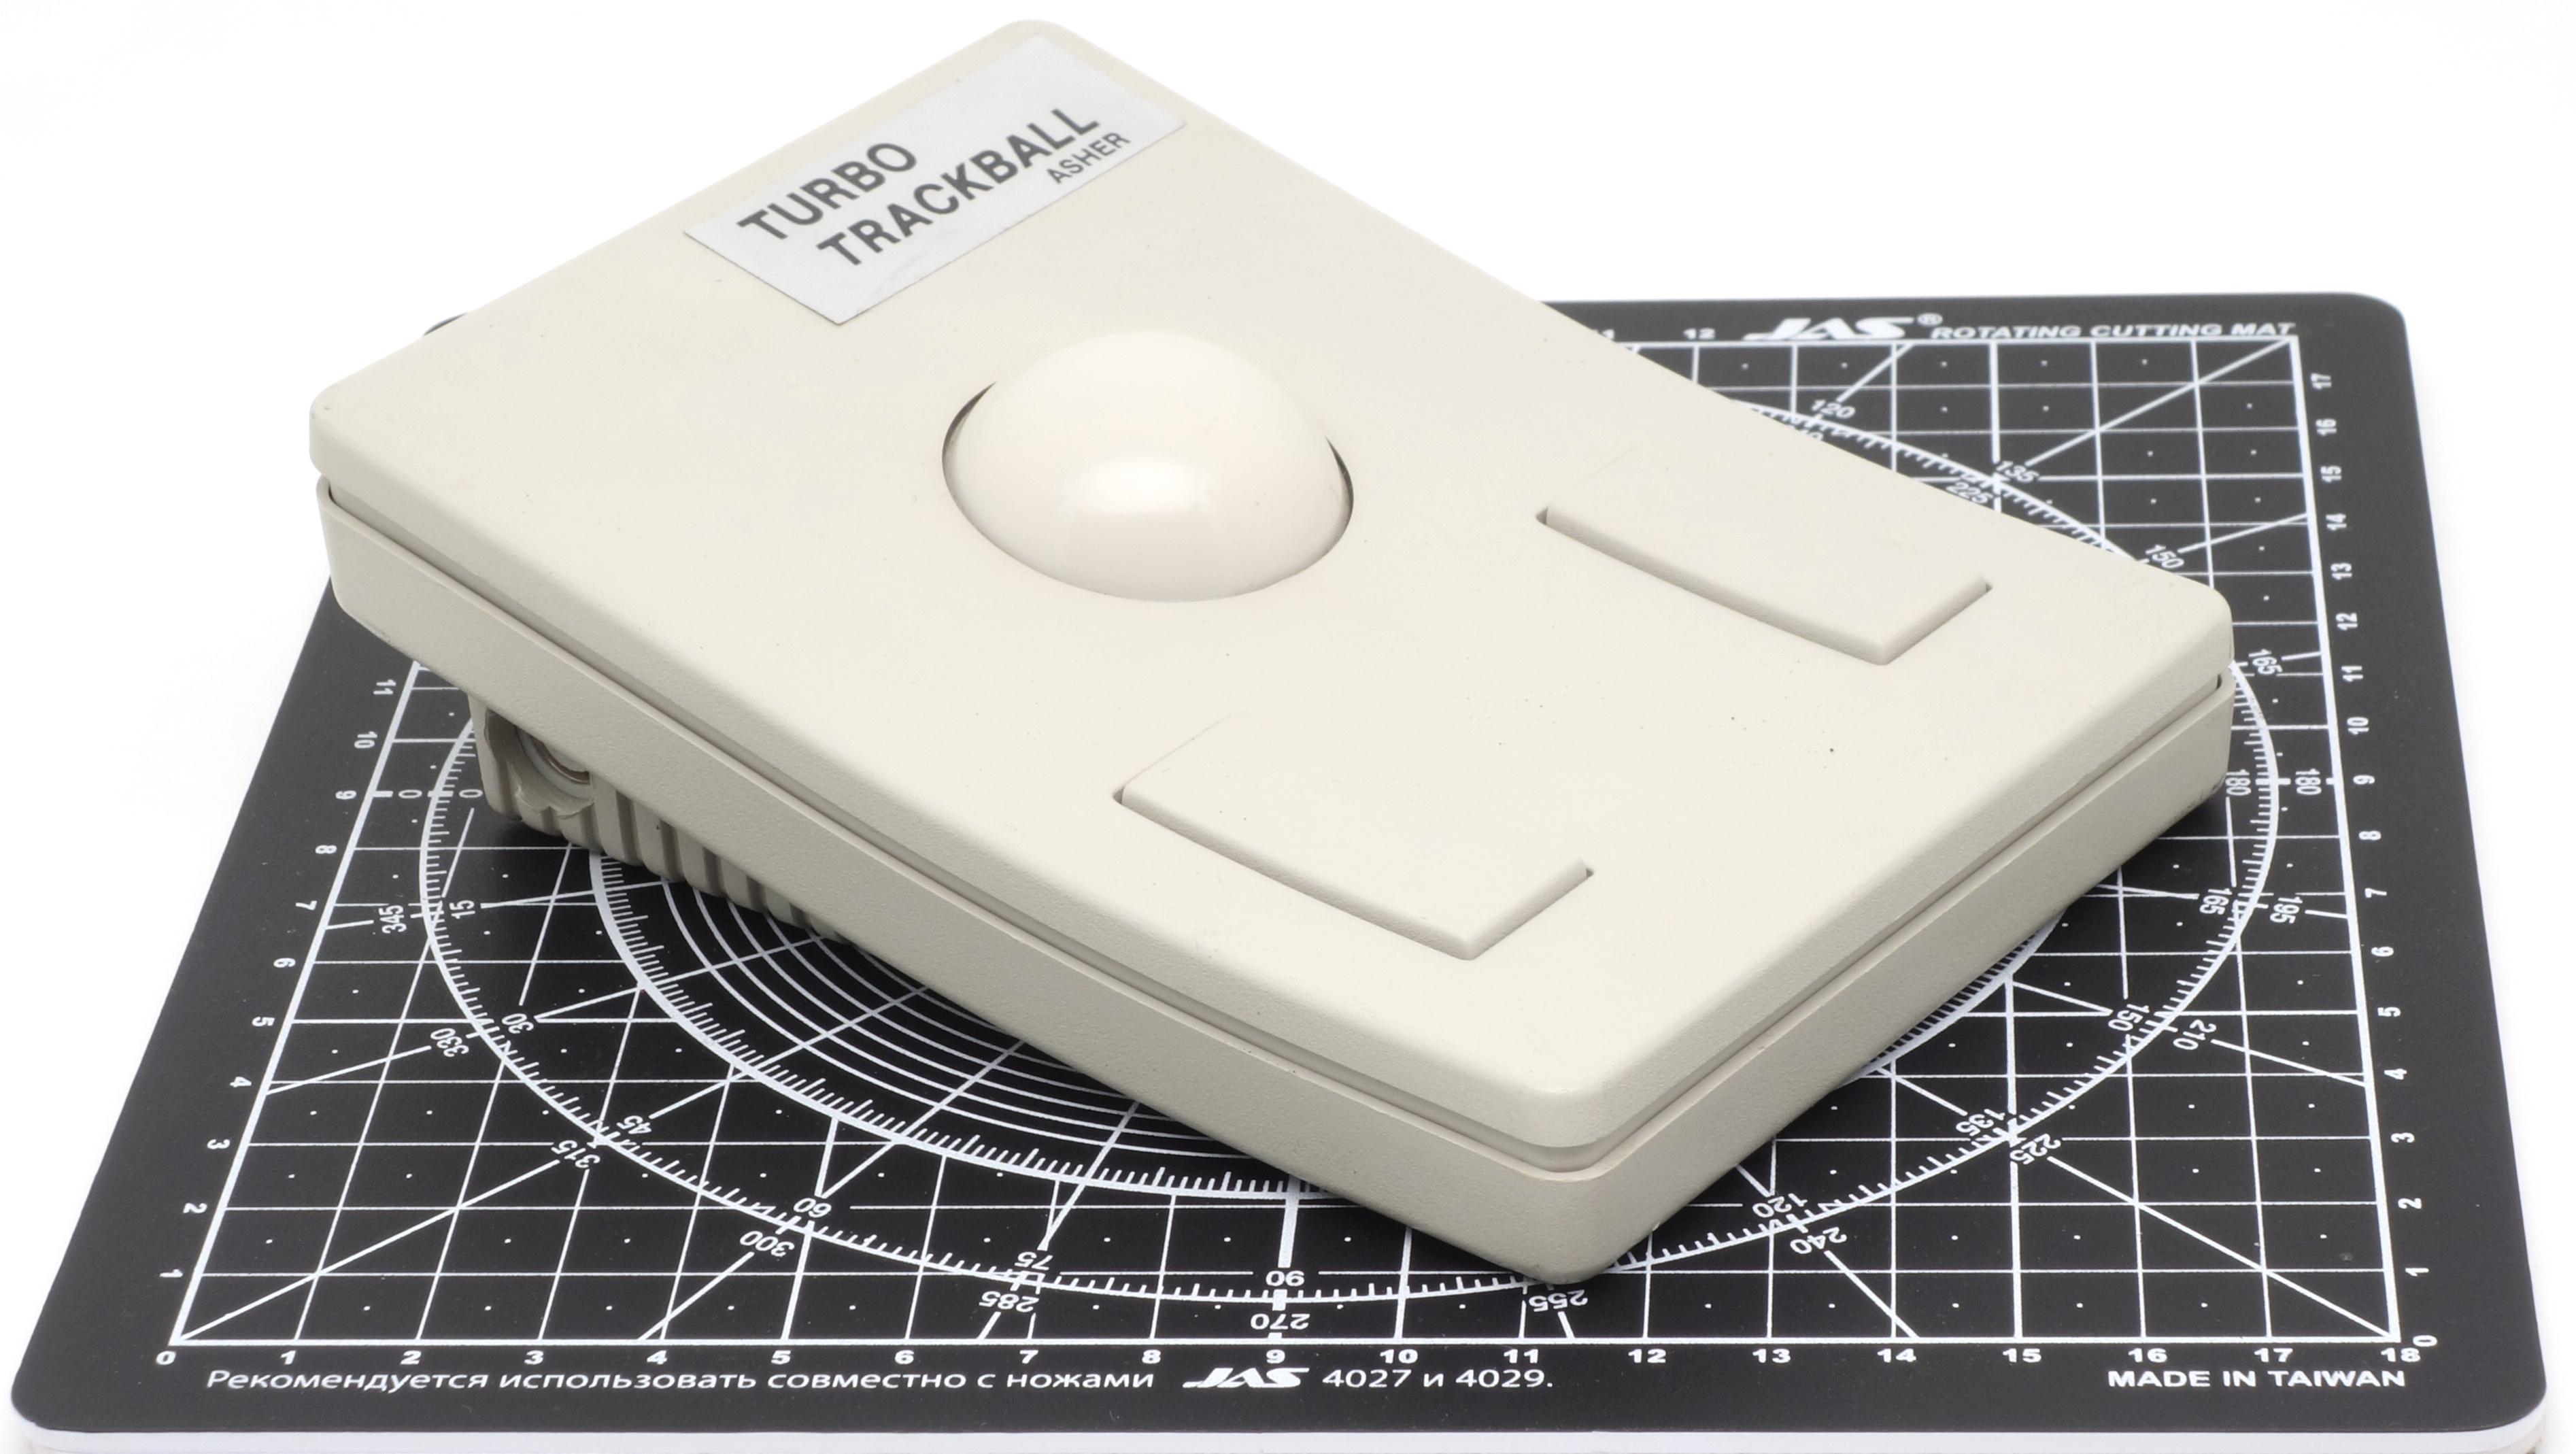
\includegraphics[scale=0.6]{1988_asher_turbo_trackball/size_30.jpg}
    \caption{Asher Turbo trackball on a graduated pad with a grid step of 1~cm}
    \label{fig:AsherSize}
\end{figure}

The trackball is symmetrical, and theoretically it can be placed to the left or right of the keyboard. Ads mention the availability of right and left hand options \cite{turbo}, but given the lack of a hardware switch, and the fact that neither long nor simultaneous button presses perform switching, the ``options'' probably refer to trackball versions, meaning that it was necessary to buy a trackball for the desired hand. In any case, in the working position, the user places index and middle fingers on the ball, while the thumb (and possibly the little finger) positions on the mouse buttons (fig. \ref{fig:AsherHand}). At the same time, unlike traditional LX200 trackballs, user's wrist rests on the table surface, just like when working with a Macintosh keyboard.

\begin{figure}[h]
    \centering
    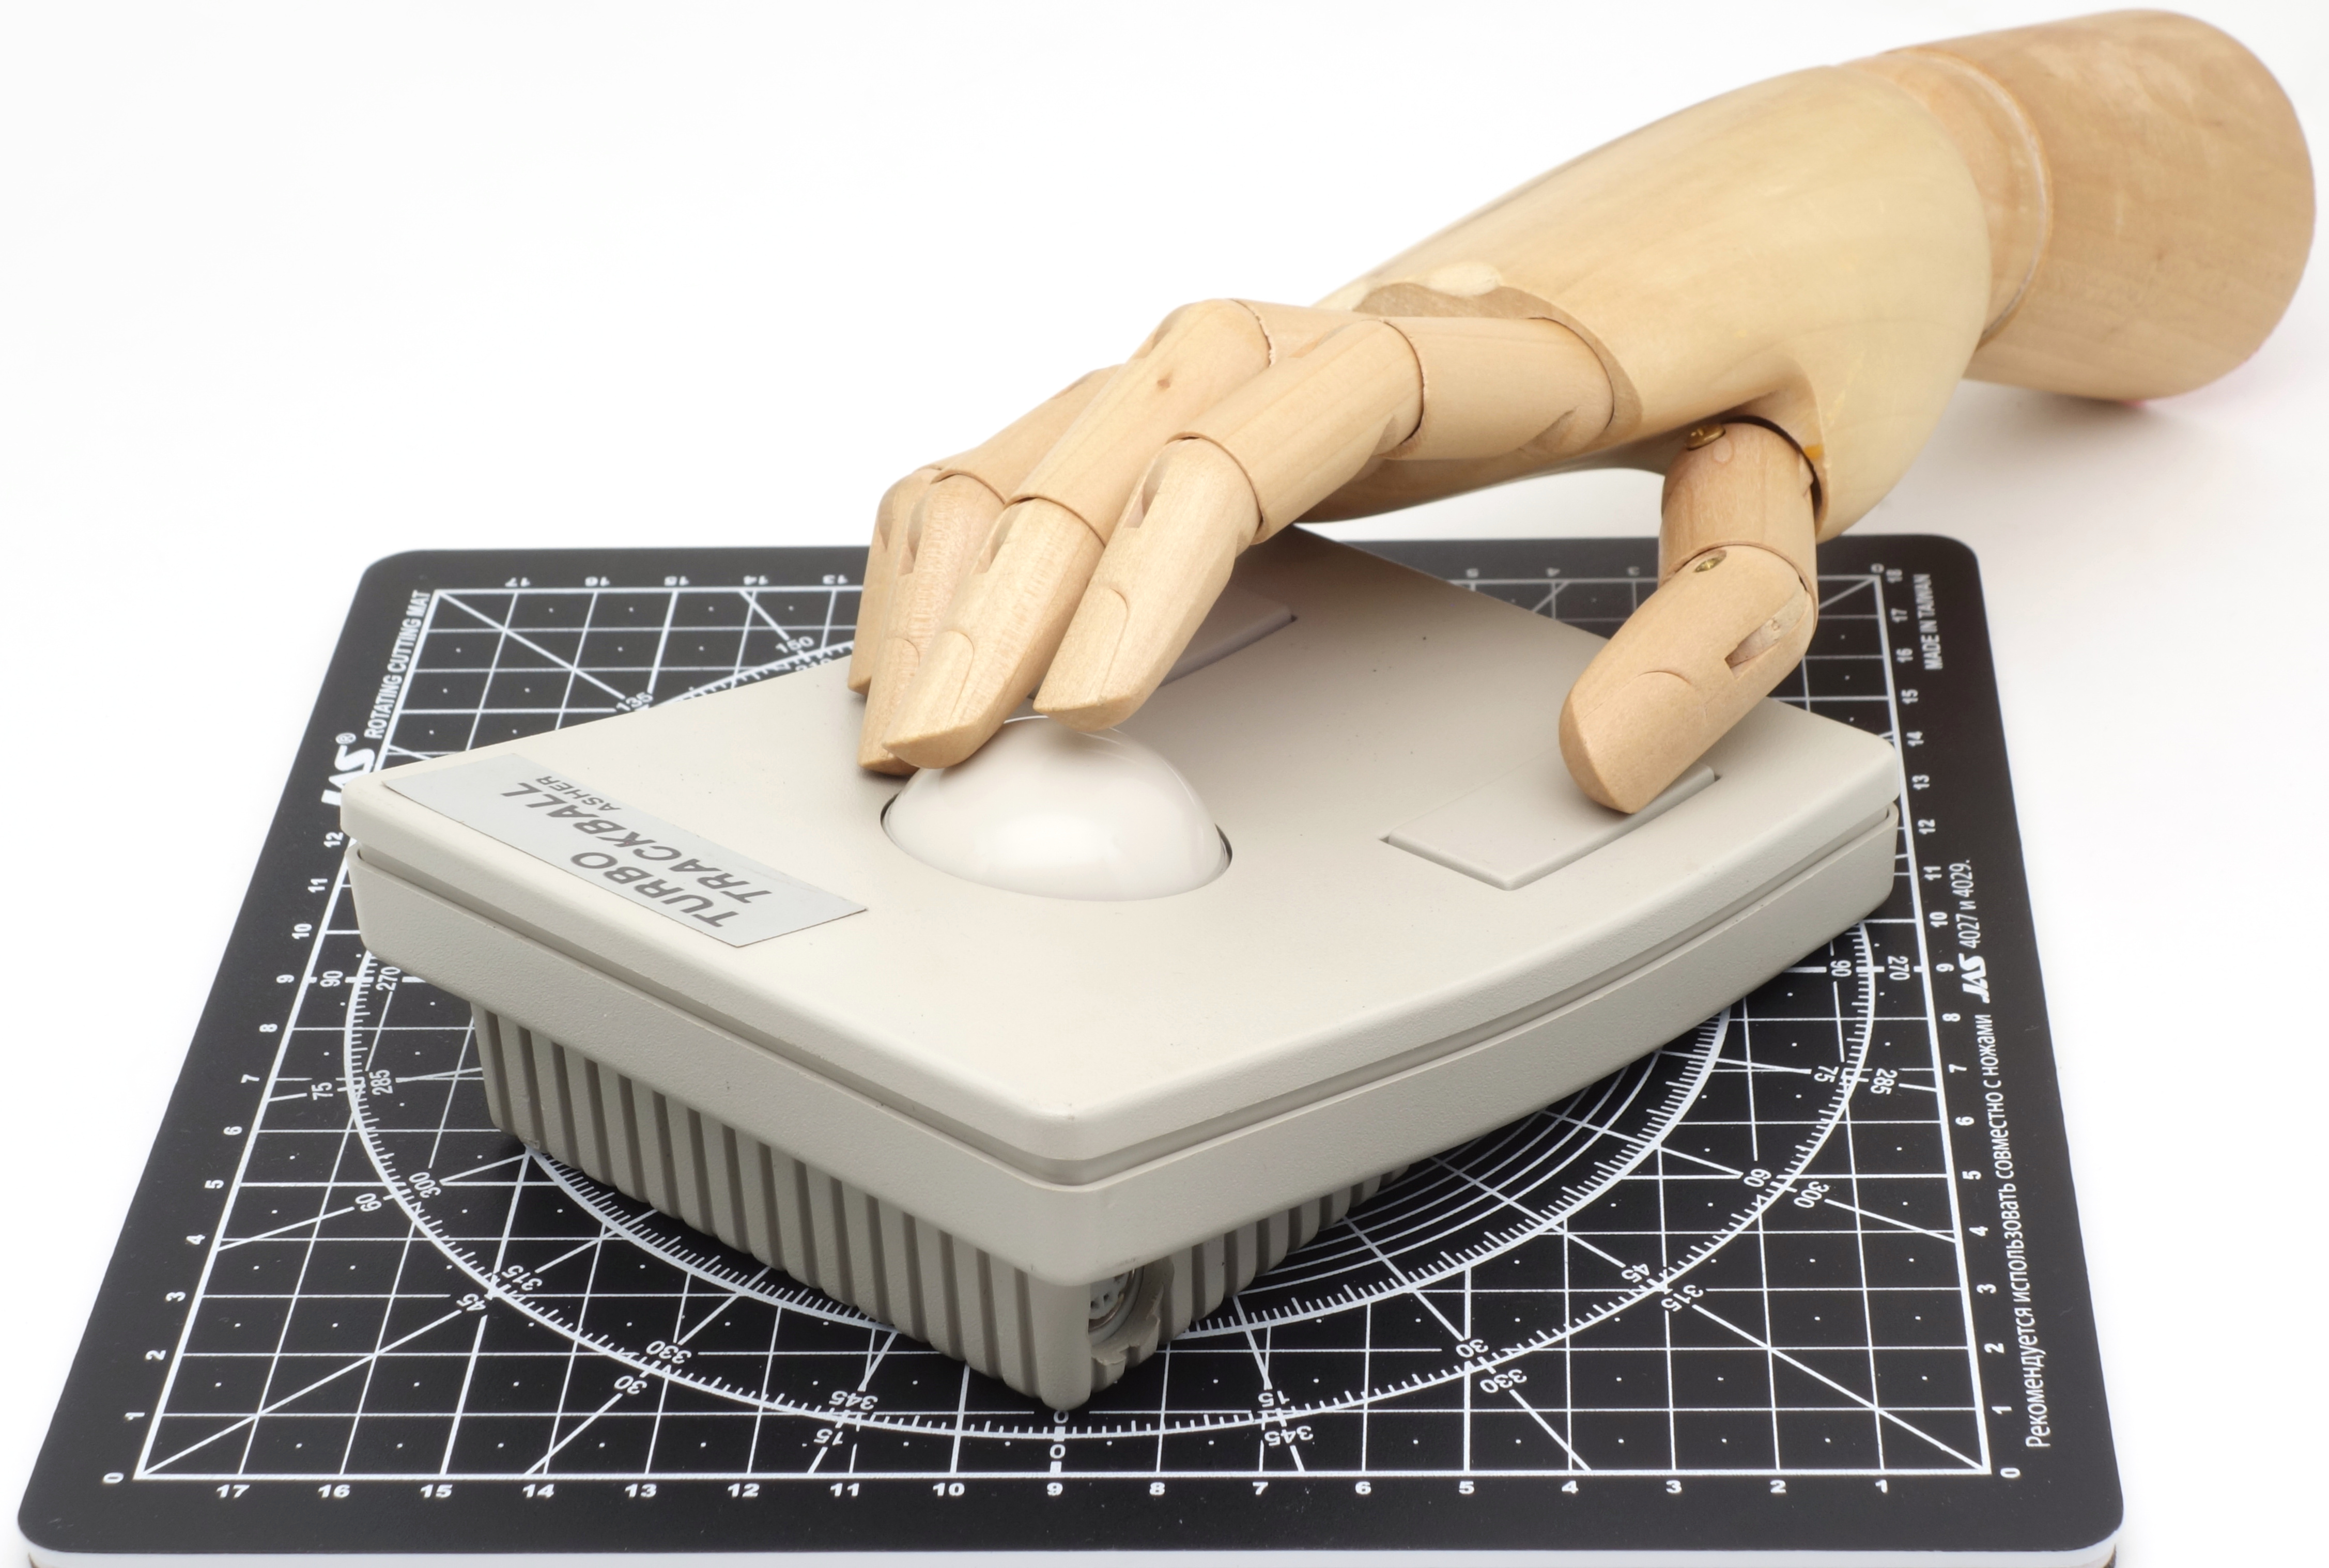
\includegraphics[scale=0.5]{1988_asher_turbo_trackball/hand_30.jpg}
    \caption{Asher Turbo trackball with a human hand model}
    \label{fig:AsherHand}
\end{figure}

Trackball internals are shown on figure \ref{fig:AsherInside}. Asher Turbo Trackball ads emphasized that, unlike its competitors, the company had its own production, and the figure clearly demonstrate this: instead of traditional casting, many elements are made using mechanical processing (milling, drilling, etc.) and soldering. In addition, the manufacturer gives a noticeable preference to composite epoxy materials traditionally used for the manufacture of printed circuit boards (judging by the appearance of individual parts, it can be assumed that they were really cut from some printed circuit boards). Finally, the ``patented hi-tech encoder'' is a regular mechanical encoder disk covered with a plastic box on top, which makes it difficult for debris to get in (however, its design is not as hermetic and is noticeably less technologically advanced compared to, for example, closed mechanical encoders from ALPS Electric, used in early models of Microsoft, IBM and some other companies' mice).

Obviously, the production of such a specific design required a significant number of manual operations, so the trackball was not produced in large batches.
The use of a mechanical encoder instead of optomechanics was probably aimed at reducing the cost of the device. Unlike the quadLYNX and other LX200 trackballs manufactured by Honeywell, similar changes affected other elements of the mechanical unit: instead of the steel bearings and shafts there are plastic rollers on a metal axis and supports cut from a composite material, which simultaneously play the role of bushings. Also, there is one more distinctive feature worth to be noted: the ball is supported by six small steel balls located in a circle, deepened in the grooves on the printed circuit board.

\begin{figure}[h]
    \centering
    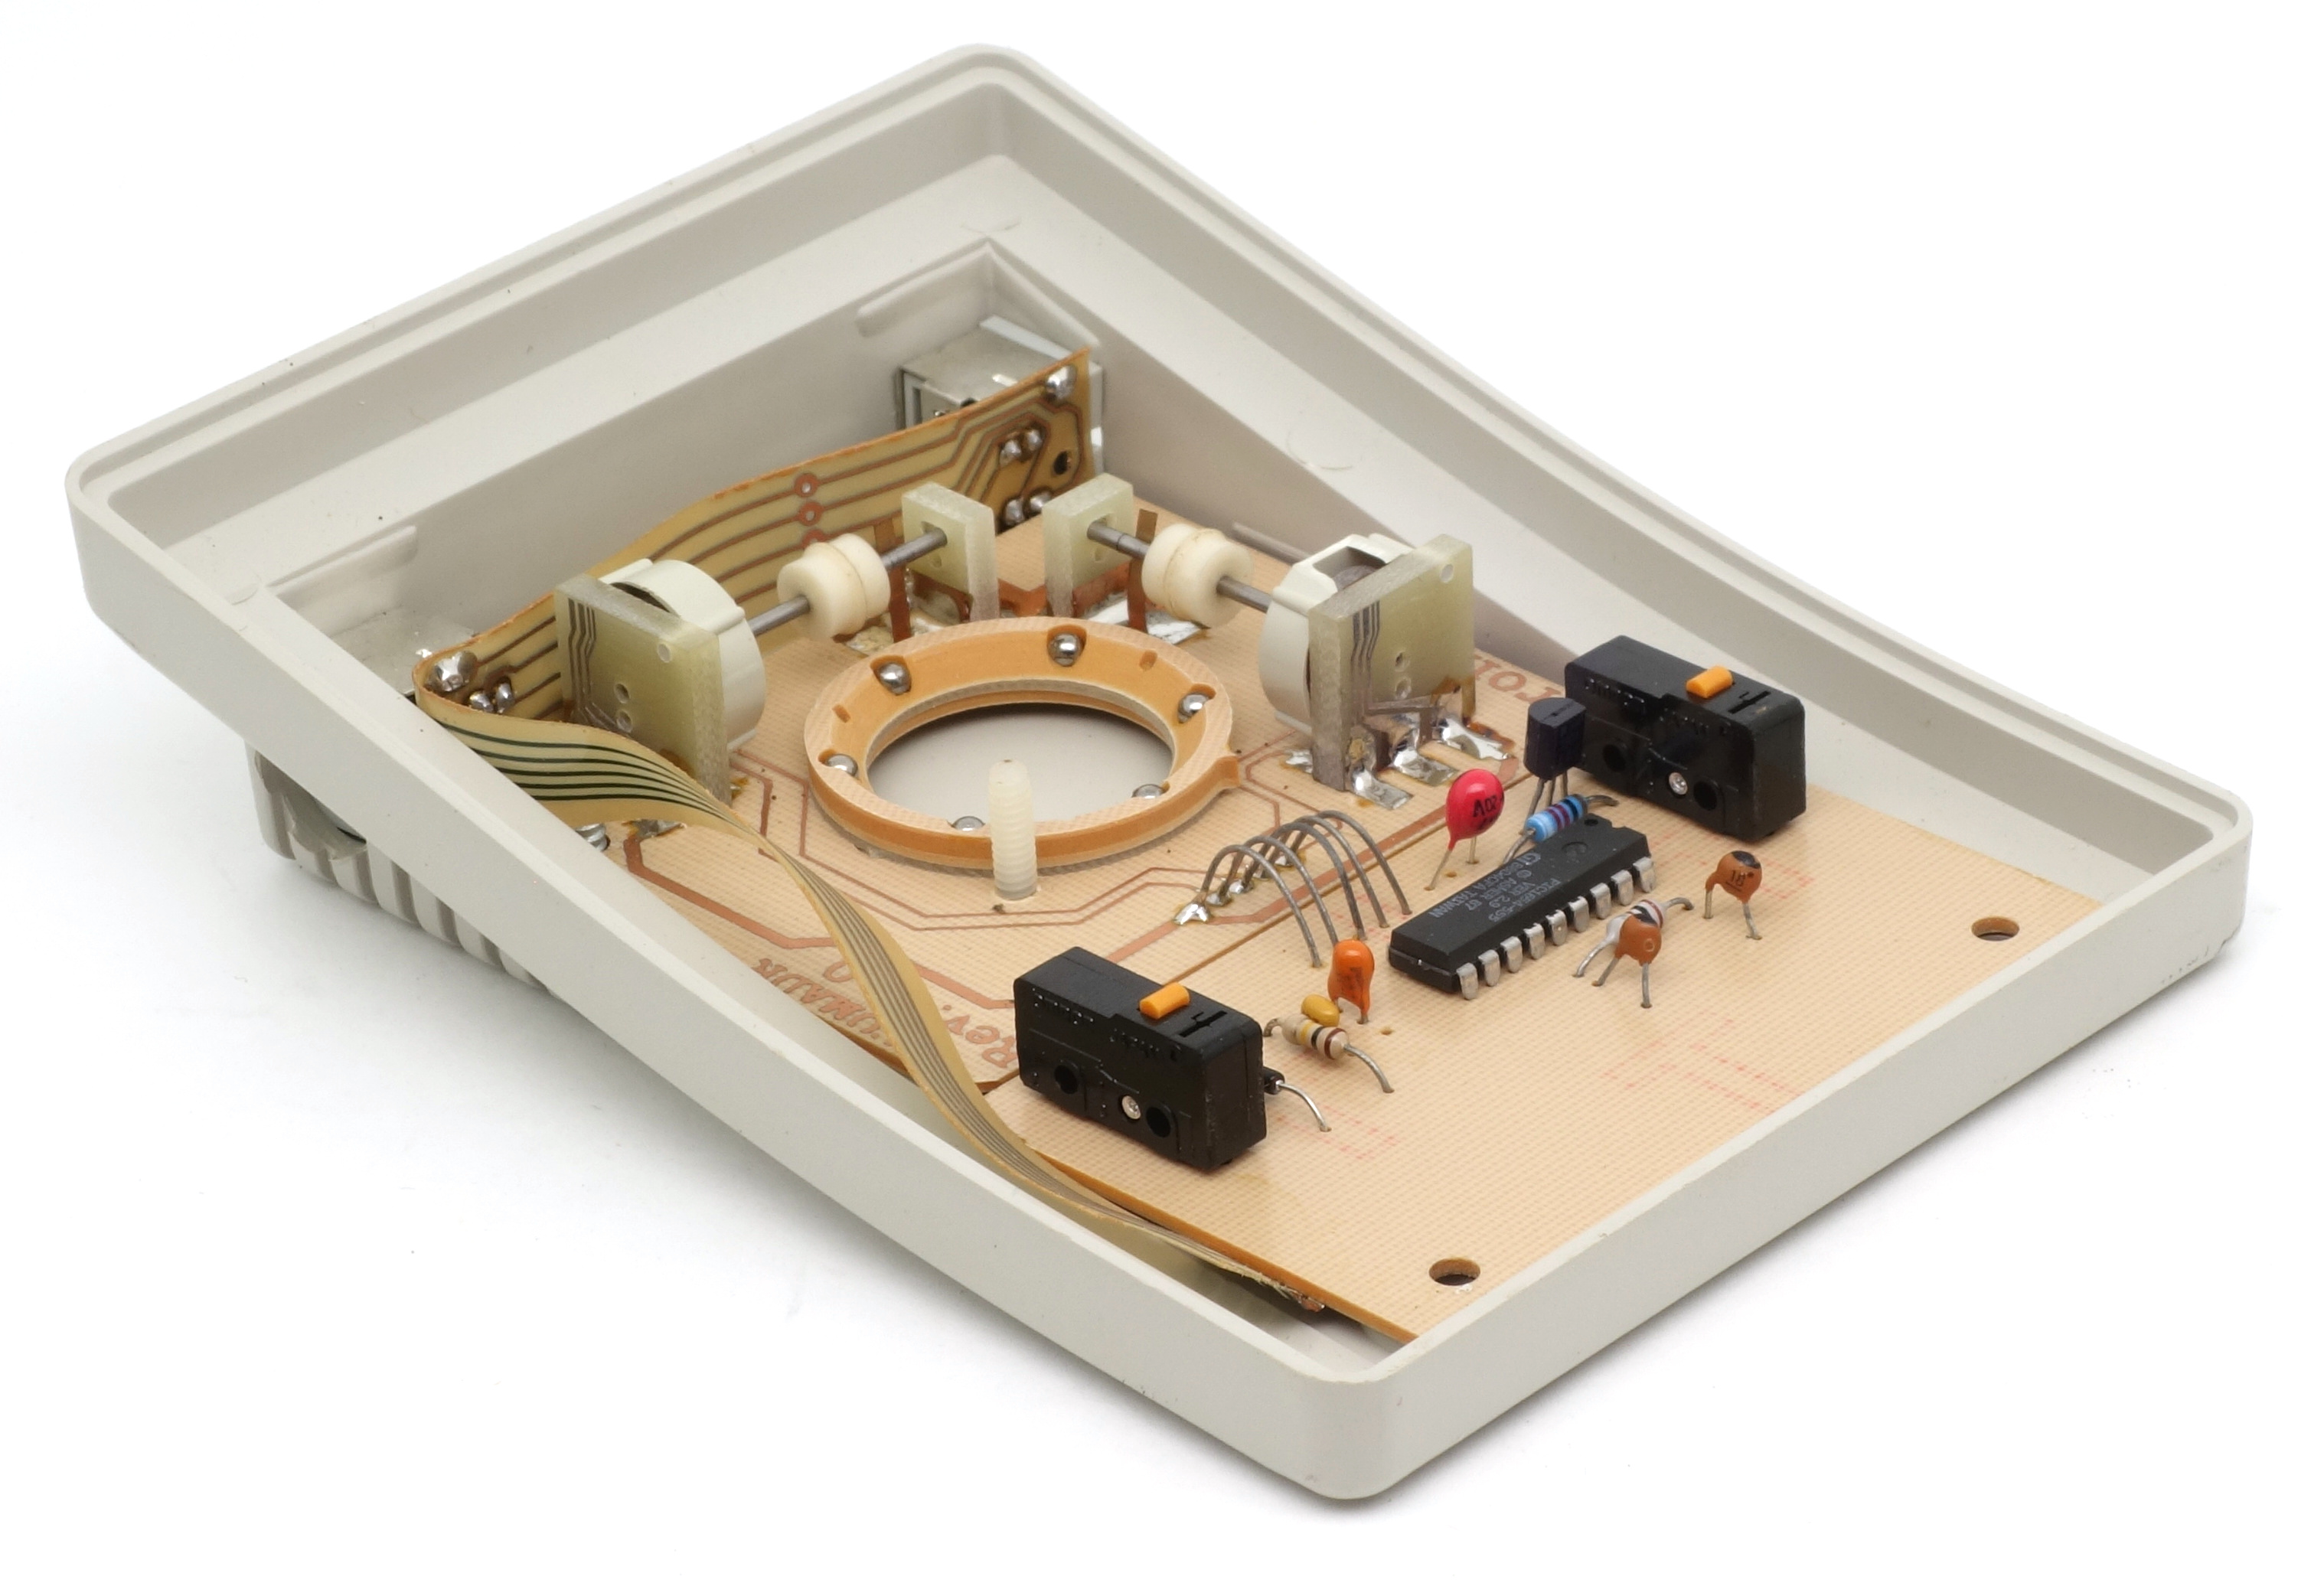
\includegraphics[scale=0.7]{1988_asher_turbo_trackball/inside_60.jpg}
    \caption{Asher Turbo trackball disassembled}
    \label{fig:AsherInside}
\end{figure}

\begin{thebibliography}{9}
\bibitem {lx200} Disc Instruments LX200 \url{https://web.archive.org/web/20220501213039/https://forum.trackballs.eu/viewtopic.php?f=17&t=16}
\bibitem {honeywell} Try the new quadLYNX Trackball // Macworld, August 1986. P. 155  \url{https://archive.org/details/eu_Macworld-1986-08_OCR/page/n155/mode/2up}
\bibitem {asher} Try the new quadLYNX Trackball // Macworld, January 1988. P. 212 \url{https://archive.org/details/macworld00unse_oel/page/212/mode/2up}
\bibitem {turbo} New Turbo Trackball from Asher // MacUser, February, 1988. P. 320 
\url{https://archive.org/details/MacUser8802February1988/page/n323/mode/2up}
\end{thebibliography}
\end{document}
